
\documentclass{article}
\usepackage{hyperref}
\usepackage{verbatim}
\usepackage[a4paper, margin=3cm]{geometry}
\usepackage{graphicx} 
\usepackage{xcolor}
\usepackage{titlesec}
\usepackage[italian]{babel}
\titleformat{\section}
  {\huge\bfseries\raggedright}
  {\thesection}{1em}{}
\titleformat{\subsection}
  {\Large\bfseries\raggedright}
  {\thesubsection}{0.8em}{}
\titleformat{\subsubsection}
  {\large\bfseries\raggedright}
  {\thesubsubsection}{0.6em}{}
\renewcommand{\theenumi}{\Roman{enumi}}

\definecolor{Sapienza}{RGB}{130, 36, 51}
\renewcommand{\contentsname}{Indice} 

\begin{document}

\begin{figure}[h]
	\centering   % Centrare l'immagine
	
\includegraphics[width=1\textwidth]{logoSapienza.png}
\end{figure}

\centering \rule{\textwidth}{0.5mm}
\paragraph{\Huge \centering \textbf{Ingegneria del Software}}
\centering \rule{\textwidth}{0.5mm}

\vspace{55pt}

\par {\Huge \centering \color{Sapienza} \textbf {Progetto Sky Watch}}

\vspace{35pt}

\par{
	\begin{figure}[h]
		\centering
		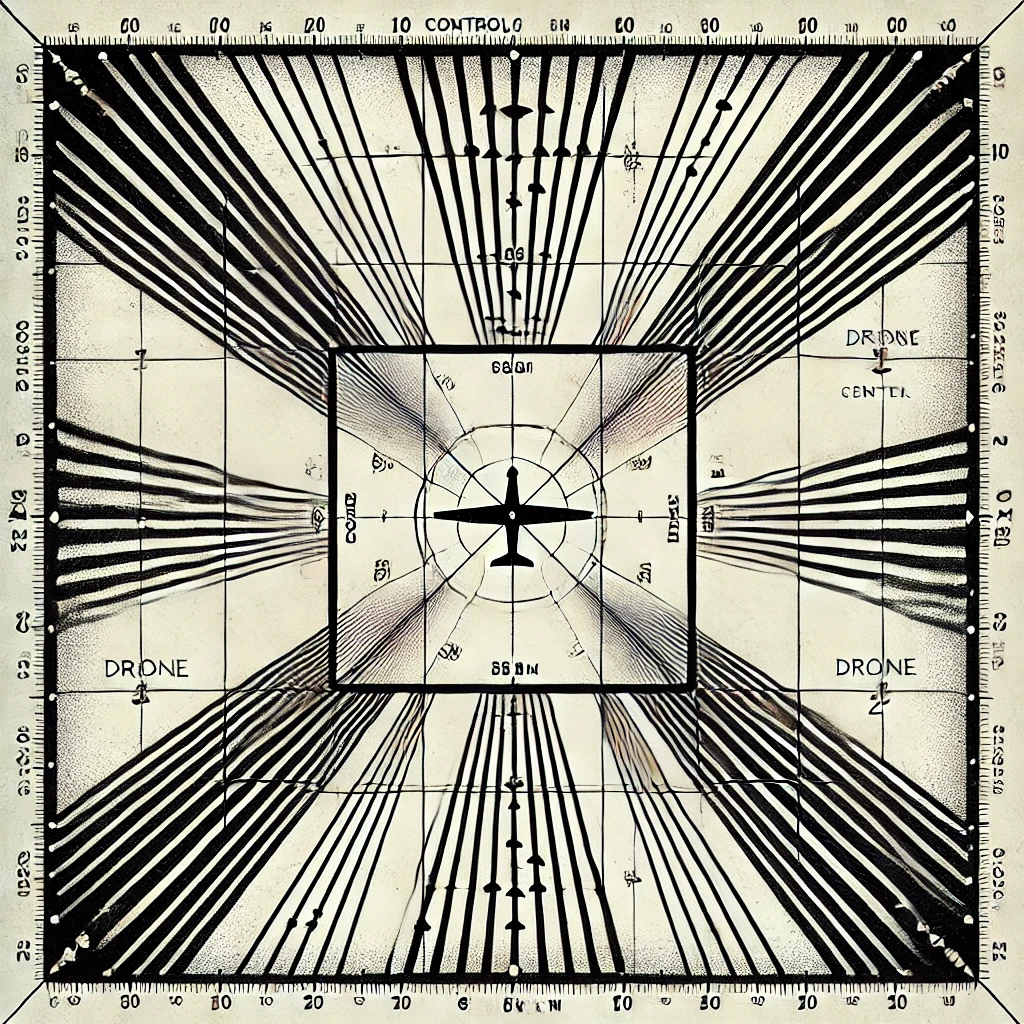
\includegraphics[width=0.5 \textwidth]{IconaSkyWatch.png}
	\end{figure}
}
\vspace{25pt}
\par{\color{gray} \large Autori \\
	\textit{\large Davide Pietragalla 1965270\\
		\large Damiano Pezzillo Iacono 1892597}
}

\newpage
\begin{large}
	\tableofcontents
\end{large}
\newpage

\section{Introduzione}
\raggedright\par{\large{
		Il progetto prevede l'implementazione di un sistema di sorveglianza per un'area di 6km\ap{2}, utilizzando droni gestiti da un \textbf{centro di controllo} situato al centro dell'area stessa.
	}}
\vspace{10pt}
\raggedright\par{\large{
		Le specifiche fornite stabiliscono che ogni \textbf{drone} abbia un'autonomia di volo di 30 minuti, un tempo di ricarica compreso tra le 2 e le 3 ore (scelto randomicamente), e che si muova alla velocità costante di 30Km/h.
	}}
\vspace{10pt}
\raggedright\par{\large{
		L'obiettivo è quello di garantire che ogni punto dell'area venga verificato almeno ogni 5 minuti.\\
		Un punto è verificato quando è presente un drone entro i 10 metri di distanza.
	}}
\vspace{10pt}
\raggedright\par{\large{
		Infine è stato richiesto un modello per i droni, un modello per il centro di controllo, una base di dati, 3 monitor di proprietà funzionali, 2 monitor di proprietà non funzionali e un'adeguata comunicazione tra i componenti.
	}}
\newpage
\section{Requisiti dell'Utente}
\raggedright\par{\large{
		Basandoci sulle specifiche del progetto siamo riusciti ad individuare i seguenti user requirements, e li abbiamo suddivisi in \textbf{requisiti funzionali}, e \textbf{requisiti non funzionali}.
	}}  \subsection{Requisiti Funzionali}
\raggedright\par{\large{
		Questa prima categoria descrive le funzionalità specifiche del sistema:
	}}
\raggedright\par{\normalsize{
		\begin{enumerate}
			\item Ogni punto dell'area deve essere verificato entro 5 minuti
			\item I droni devono avere un raggio di verifica di 10 metri
			\item Il centro di controllo deve gestire i droni
			\item Ogni ricarica deve avere una durata presa casualmente tra le 2 e le 3 ore
			\item Il sistema deve registrare in un database tutte le informazioni rilevanti
			\item L'utente deve poter vedere la percentuale di coverage attuale
			\item L'utente deve poter avviare e terminare il sistema
		\end{enumerate}
	}}
\subsection{Requisiti Non Funzionali}
\raggedright\par{\large{
		In secondo luogo abbiamo i requisiti che riguardano le prestazioni, l'affidabilità e altri aspetti qualitativi:
	}}
\raggedright\par{\normalsize{
		\begin{enumerate}
			\item Il sistema deve essere in grado di mantenere un certo grado di affidabilità ed economicità
			\item Una volta raggiunto il 100\% del coverage, il sistema deve essere in grado di mantenerlo fino alla terminazione
			\item Ogni drone deve tornare alla base di ricarica prima di esaurire la propria autonomia
			\item Il centro di controllo e la base di ricarica devono trovarsi al centro dell'area
		\end{enumerate}
	}}
\subsection{UML degli Use Case}
\raggedright\par{\large{
		Segue la rappresentazione in UML (Unified Modeling Language) degli Use Case, diagrammi che descrivono le interazioni tra un sistema e i suoi utenti:
	}}
\par{
	\begin{figure}[h]
		\centering   % Centrare l'immagine
		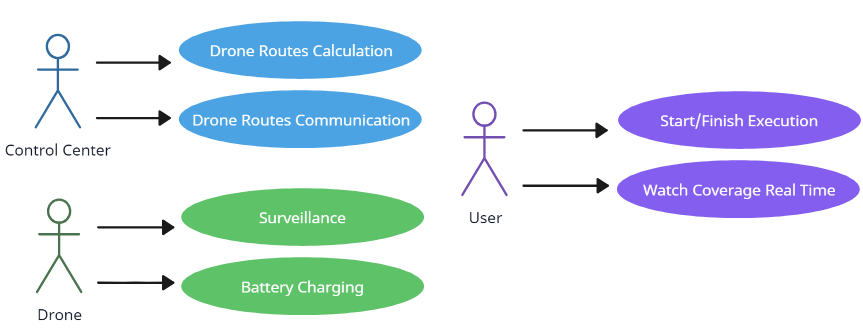
\includegraphics[width=1\textwidth]{UseCase.png}
	\end{figure}
}
\newpage
\section{Requisiti del Sistema}
\raggedright\par{\large{
		In modo analogo al capitolo precedente, abbiamo individuato alcuni requisiti del sistema.
	}}
\subsection{Requisiti Funzionali}\label{sec:Funzionali}
\raggedright\par{\large{
		Le funzionalità specifiche che il sistema deve offrire per soddisfare validità e integrità:
	}}
\raggedright\par{\normalsize{
		\begin{enumerate}
			\item Il centro di controllo deve calcolare le rotte dei droni
			\item Il centro di controllo deve inoltrare le rotte ai droni
			\item Il centro di controllo deve ricevere le informazioni necessarie dai droni
			\item Il centro di controllo deve stabilire se un punto non è stato verificato entro 5 minuti
			\item Il drone deve ricevere la rotta dal centro di controllo
			\item Il drone deve essere inserito tra i droni disponibili una volta terminata la ricarica
			\item Il centro di controllo deve registrare nel database i dati di una sessione
		\end{enumerate}
	}}
\subsection{Requisiti Non Funzionali}\label{sec:NonFunzionali}
\raggedright\par{\large{
		Le qualità e le prestazioni che il sistema deve mantenere, come usabilità, affidabilità e scalabilità:
	}}
\raggedright\par{\normalsize{
		\begin{enumerate}
			\item Il sistema deve essere in grado di ottenere un coverage del 100\% con un massimo di 9000 droni
			\item La comunicazione tra i vari componenti avviene tramite stream Redis
			\item Le connessioni redis non devono superare le 10.000 unità
			\item La lunghezza degli stream non deve superare la soglia di 4000 messaggi
			\item I dati rilevanti verranno registrati in un database PostgreSQL
			\item Generazione e invio delle query inerenti la reportiva deve concludersi nel giro di un secondo
		\end{enumerate}
	}}
\subsection{Architettura del Sistema}
\raggedright\par{\large{
		Lo schema illustra i componenti principali del sistema e le interazioni fra di essi:
	}}
\par{
	\begin{figure}[h]
		\centering   % Centrare l'immagine
		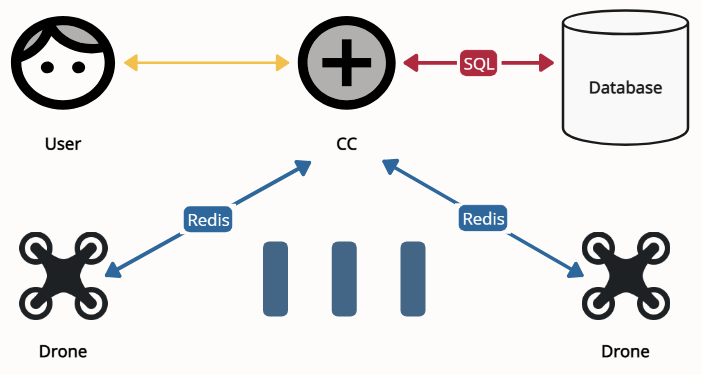
\includegraphics[width=0.6\textwidth]{Architettura.png}
	\end{figure}
}
\newpage
\subsection{Activity Diagram}
\raggedright\par{\large{
		Il seguente diagramma fornisce una rappresentazione del flusso di esecuzione del centro di controllo e dei droni dall'inizio alla fine dell'applicazione:
	}}
\par{
	\begin{figure}[h]
		\centering
		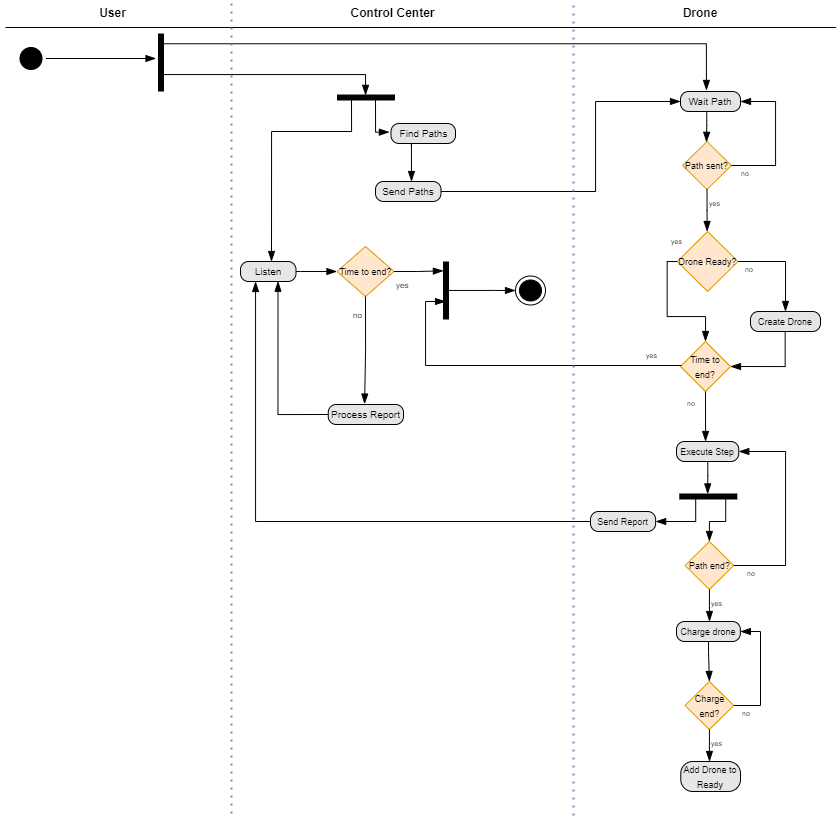
\includegraphics[width=1\textwidth]{ActivityDiagram.png}
	\end{figure}
}
\newpage
\subsection{State Diagrams}
\raggedright\par{\large{
		Una rappresentazione degli stati del centro di controllo e delle transizioni tra di essi in base ai possibili eventi:
	}}
\par{
	\begin{figure}[h]
		\centering
		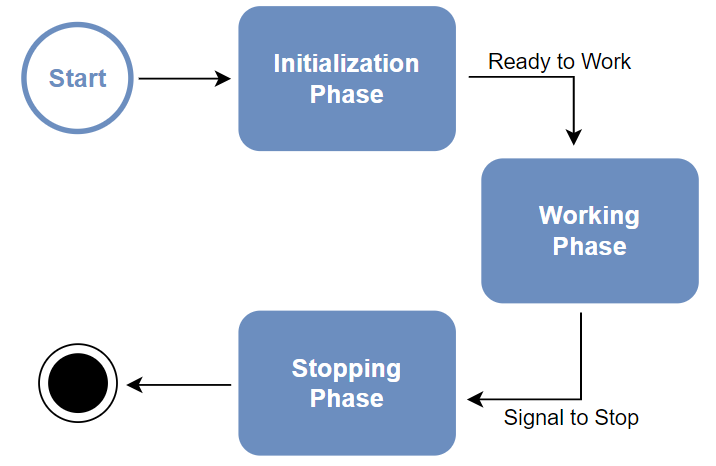
\includegraphics[width=0.5\textwidth]{CCSD.png}
	\end{figure}
}
\raggedright\par{\large{
		Una rappresentazione degli stati dei droni e delle transizioni tra di essi in risposta ai vari eventi e condizioni possibili:
	}}
\par{
	\begin{figure}[h]
		\centering   % Centrare l'immagine
		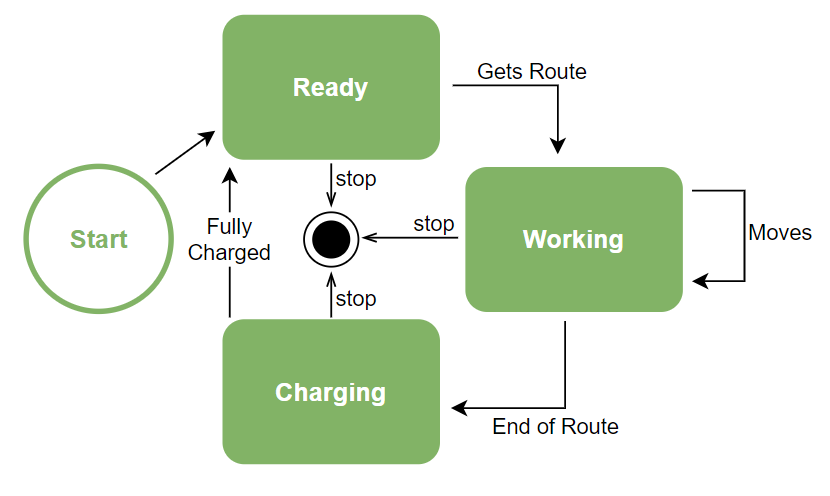
\includegraphics[width=0.5\textwidth]{DroneSD.png}
	\end{figure}
}
\subsection{Message Sequence Chart}
\raggedright\par{\large{
		Questo grafico raffigura lo scambio di messaggi che avviene per l'ottenimento di una lista di monitor\_failure:
	}}
\par{
	\begin{figure}[h]
		\centering   % Centrare l'immagine
		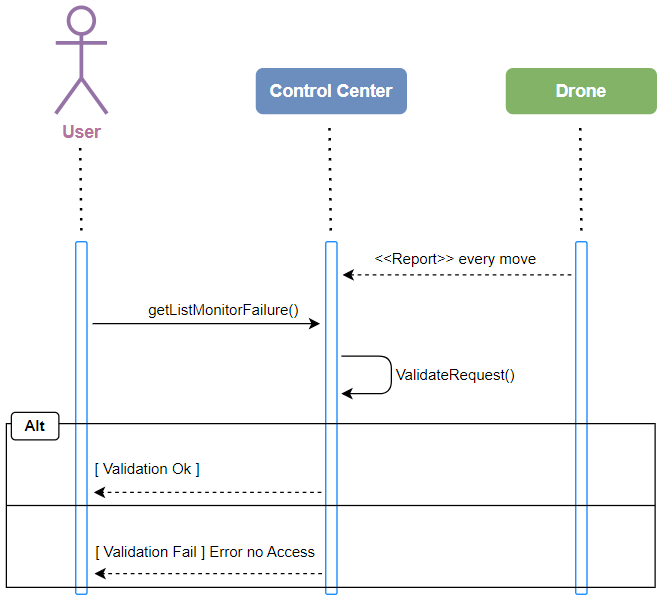
\includegraphics[width=0.55\textwidth]{MessageSequenceChart.png}
	\end{figure}
}
\newpage
\section{Implementazione}
\subsection{Strategia Sfruttata}
\raggedright\par{\large{
		La strategia che il centro di controllo utilizza per calcolare il percorso dei droni e garantire una copertura ottimale, consiste nell'indicare a ciascun drone un punto strategico dove iniziare la sua ronda.
	}}
\vspace{10pt}
\raggedright\par{\large{
		Il drone proseguirà verso est quando la coordinata Y è pari, e verso ovest quando è dispari, spostandosi verso il basso una volta raggiunto il limite dell'area; inoltre se il drone arriva ad avere l'autonomia sufficiente per tornare al centro di controllo, procede a ritirarsi.
	}}
\vspace{10pt}
\raggedright\par{\large{
		I punti strategici partono dalle coordinate (0,0), e vengono aggiunti quei punti a cui la ronda precedente non può arrivare per via della batteria.
	}}
\vspace{10pt}
\raggedright\par{\large{
		Ogni drone poco prima che passino 5 minuti dalla partenza, invia un segnale di richiesta di copertura, e un altro drone parte sfruttando lo stesso percorso del padre. Questo garantisce la verifica dell'area entro i 5 minuti poiché i droni hanno tutti una velocità costante di 30Km/h.
	}}
\subsection{Algoritmi Utilizzati}
\vspace{5pt}
\raggedright\par{\large{
		\begin{verbatim}
Class Control_Center{
    public:
    
    Control_Center():
	       determino la dimensione del CC
	       stabilisco una connessione con il DB postgres
	       creo una nuova sessione nel DB
	       inizializzo la griglia che rappresenta l’area
	
    updateGrid(x, y):
	       aggiorno l’ultima visita del punto (x, y) al tempo corrente

    getTimeFromGrid(x, y):
        restituisco il momento dell’ultima visita del punto (x, y) 

    executeQuery(query):
	       stabilisco un lock sul mutex delle query
	       eseguo la query di creazione o modifica
	       sblocco il mutex

    getValueQuery(query, row, column):
	       prendo il risultato di una query tramite getTuples(query)
	       restituisco il valore alla riga row e colonna column




    getTuples(query):
	       stabilisco un lock sul mutex delle query
        eseguo la query di lettura
	       sblocco il mutex
	       restituisco il risultato

    getSessionId():
	       restituisce l’id della sessione

    getCCId():
	       restituisce l’id del CC
}

    goTo(x, y, nx, ny):
	       crea una stringa vuota
	       aggiunge l se da (x, y) a (nx, ny) serve andare a sinistra
        aggiunge r se da (x, y) a (nx, ny) serve andare a destra
        aggiunge u se da (x, y) a (nx, ny) serve andare su
        aggiunge d se da (x, y) a (nx, ny) serve andare giu
        aggiorna (x, y)
        ripeti finche (x, y) = (nx, ny)
        restituisco la stringa ottenuta

    goToGridX(x, y, step):
	       creo una stringa vuota
	       procedo andando a destra se y è pari e aggiungo r
	       procedo andando a sinistra se y è dispari e aggiungo l
	       se mi trovo al limite della riga vado giù e aggiungo d
	       decremento di uno step
	       ripeto finché step = mosse necessarie per tornare a (150, 150)
	       utilizzo goTo() per tornare al punto (150, 150)
	       concateno le stringhe in una
	       restituisco la stringa

    findPaths(paths, cc):
	       inizializzo x, y a 0
	       inizializzo un vettore di stringhe
	       utilizzo goTo() per posizionare il drone
	       utilizzo goToGrid() per calcolare il restante percorso
        aggiungo la stringa ottenuta al vettore
        ripeto fino alla completa visita della griglia
        restituisco il vettore

    doQuery(cc, query):
        esegue cc.executequery(query) 



    listenDronesX(cc):
	       ascolta i report dei droni
	       preso un report esegue il check di:
	       CC_OVERLOAD
	       MISSING_REPORT
	       AREA_COVERAGE
	       ad ogni report aggiorna le informazioni di cc
	       termina quando stopflag diventa true

    timer():
	       rende stopflag true allo scadere di un tot di secondi

    periodicReport():
	       stampa un report di cc periodicamente

Class Drone{
    public
    
    Drone():
        costruttore drone

    ExecuteMove(char move):
        chiama una delle funzioni relative al movimento 

    moveLeft():
	       aggiorna il campo x del drone 

    moveUp():
		      aggiorna il campo y del drone

    moveRight():
		      aggiorna il campo x del drone 

    moveDown():
		      aggiorna il campo y del drone

    fillMovesLeft():
	       inizializza il campo moves_left ad una costante

    getRecharginTime():
	       restituisce il valore del campo recharging_time

    getMovesLeft():
	       restituisce il valore del campo moves_left

    getX():
	       restituisce il valore del campo x

    getY():
	       restituisce il valore del campo y

    getId():
	       restituisce il valore del campo id
}

    add_to_ready(Drone drone):
        inserisce il drone dato in argomento nei ready

    chargeDrone(Drone):
	       simula il processo di ricarica
	       chiama fillMovesLeft() sul drone in argomento
	       chiama add_to_ready() sul drone in argomento

    getDrone():
		      restituisce un drone dal vettore dei ready se ce ne sono 
        altrimenti ne restituisce uno nuovo

    initDroneX():
        fa eseguire al drone le mosse descritte dal path ricevuto dal CC
	       chiama i droni di copertura ogni 124 mosse
	       quando il drone conclude il suo path esegue chargeDrone()
    \end{verbatim}
	}}
\subsection{Database}
\raggedright\par{\large{
		Segue una rappresentazione del database implementato in \textbf{UML}:
	}}
\par{
	\begin{figure}[h]
		\centering
		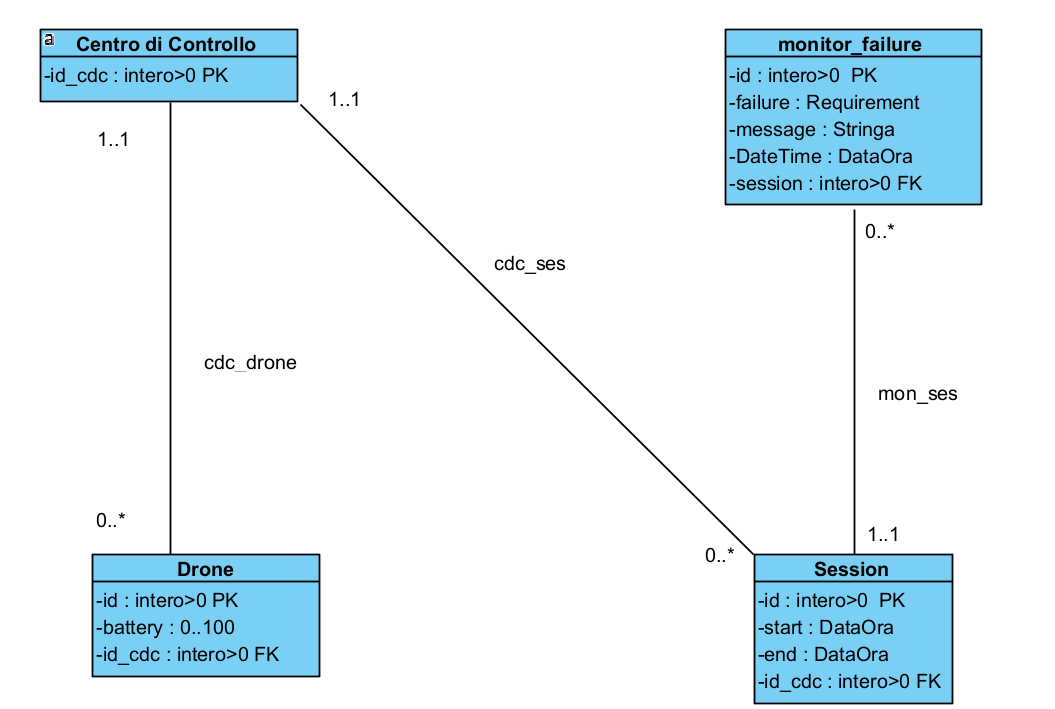
\includegraphics[width=0.8\textwidth]{UML_DB.PNG}
	\end{figure}
}
\newpage
\subsection{Connessioni Redis}
\raggedright\par{\large{
		Abbiamo usato gli \textbf{stream} di \textbf{Redi}s per far comunicare centro di controllo e droni:\\
		- Avviene una prima comunicazione affinché il CC fornisca i percorsi ai droni.\\
		- I droni ad ogni mossa che eseguono, inviano un messaggio contenente la loro\\
		\ \ nuova posizione.\\
		- Al termine dell'esecuzione il main dei droni fornisce il numero esatto di droni\\
		\ \ utilizzato al CC.
	}}
\subsection{Monitor}
\raggedright\par{\large{
		Abbiamo implementato 3 monitor di requisiti funzionali e 2 di requisiti non funzionali, i quali eseguono un insert nel database al verificarsi del problema:\\
		- \hyperref[sec:Funzionali]{\texttt{PATH\_CALCULATION}: riferito al requisito di sistema funzionale I.}\\
		- \hyperref[sec:Funzionali]{\texttt{MISSING\_REPORT}: riferito al requisito di sistema funzionale III.}\\
		- \hyperref[sec:Funzionali]{\texttt{AREA\_COVERAGE}: riferito al requisito di sistema funzionale IV.}\\
		- \hyperref[sec:NonFunzionali]{\texttt{NUM\_DRONES}: riferito al requisito di sistema non funzionale I.}\\
		- \hyperref[sec:NonFunzionali]{\texttt{CC\_OVERLOAD}: riferito al requisito di sistema non funzionale IV.}
	}}
\newpage
\section{Test e Conclusioni}
\subsection{Test}
\raggedright\par{\large{
		Al termine dell'implementazione è stato fatto un test volto a determinare il tempo che impiegano i droni per fornire una \textbf{copertura massimale} dell'area, e per determinare se tale risultato viene effettivamente mantenuto nel tempo.\\
		Il test (durato 12 ore) ha prodotto i seguenti risultati:
	}}
\par{
	\begin{figure}[h]
		\centering
		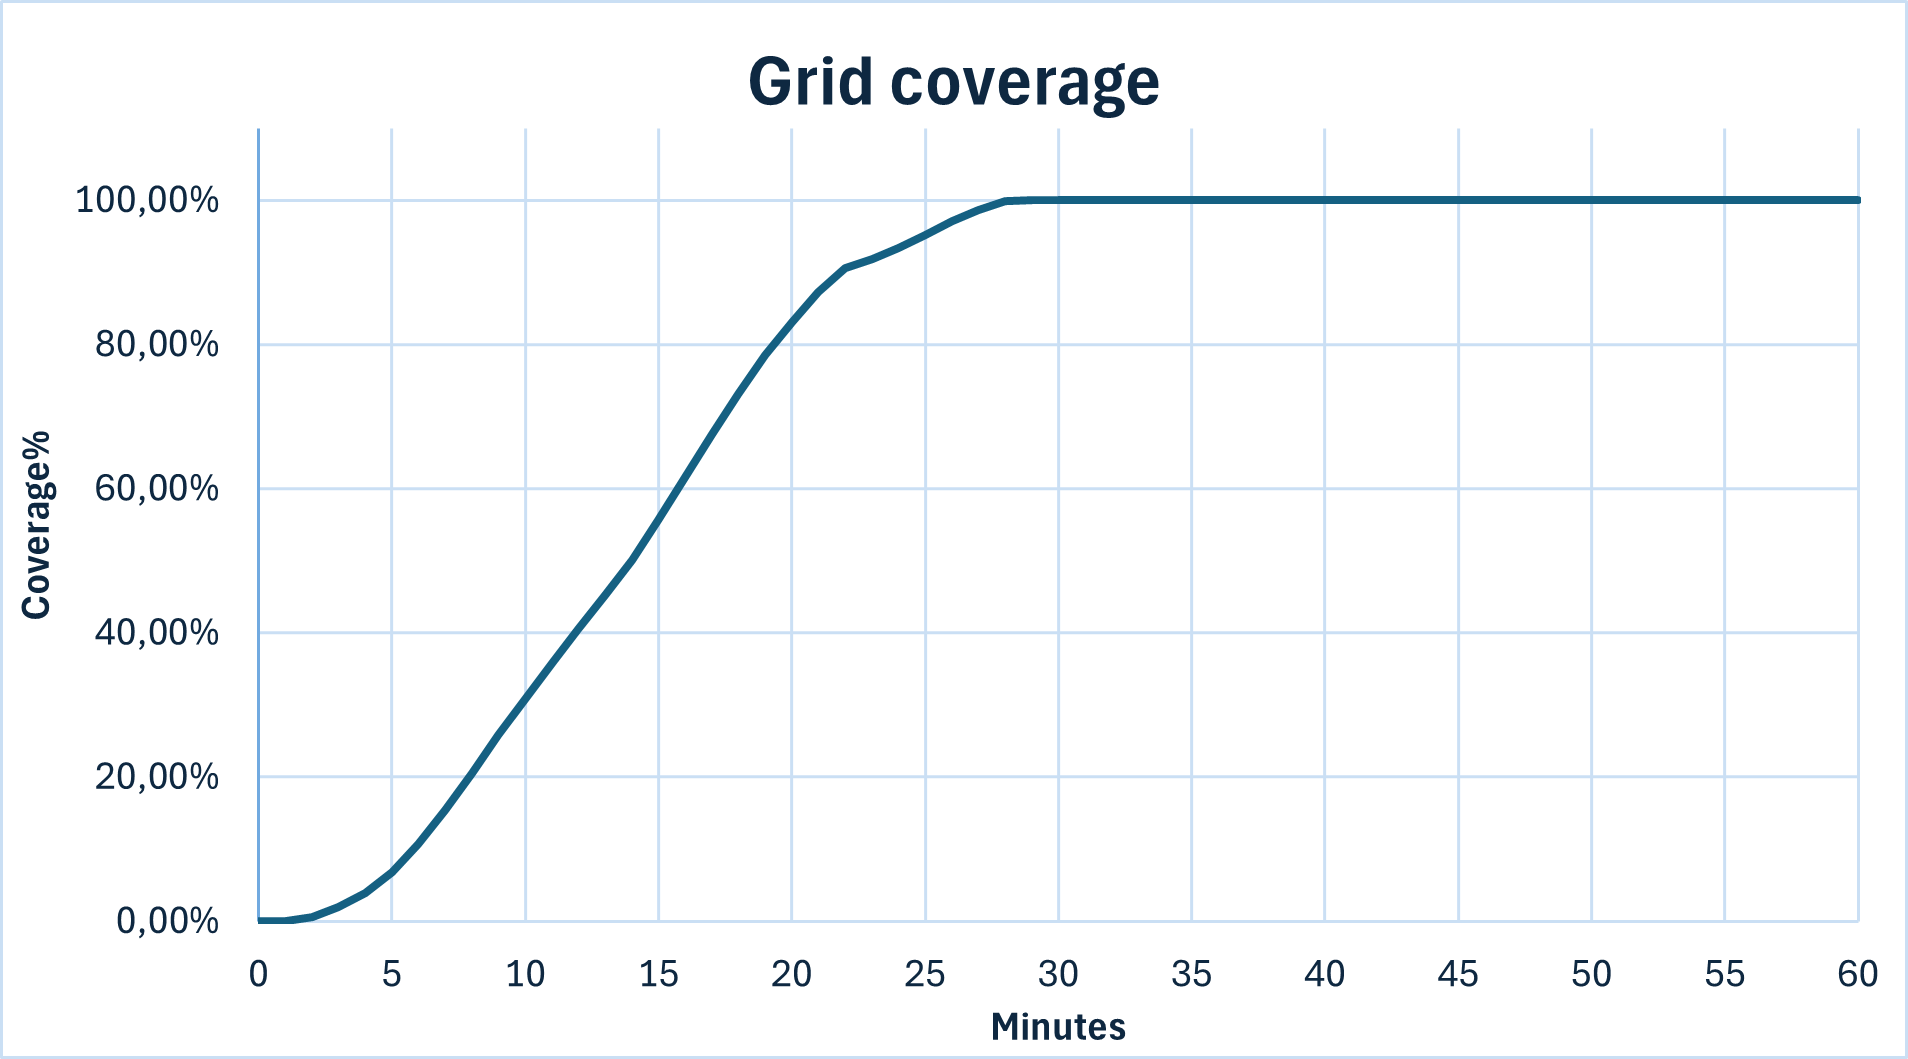
\includegraphics[width=0.9\textwidth]{grid_cov.png}
	\end{figure}
}
\vspace{20pt}
\raggedright\par{\large{
		Un ulteriore test svolto ha consentito di individuare i \textbf{droni necessari} per il raggiungimento di uno stato di \textbf{riciclo perpetuo}, in base al tempo medio di ricarica:
	}}
\par{
	\begin{figure}[h]
		\centering
		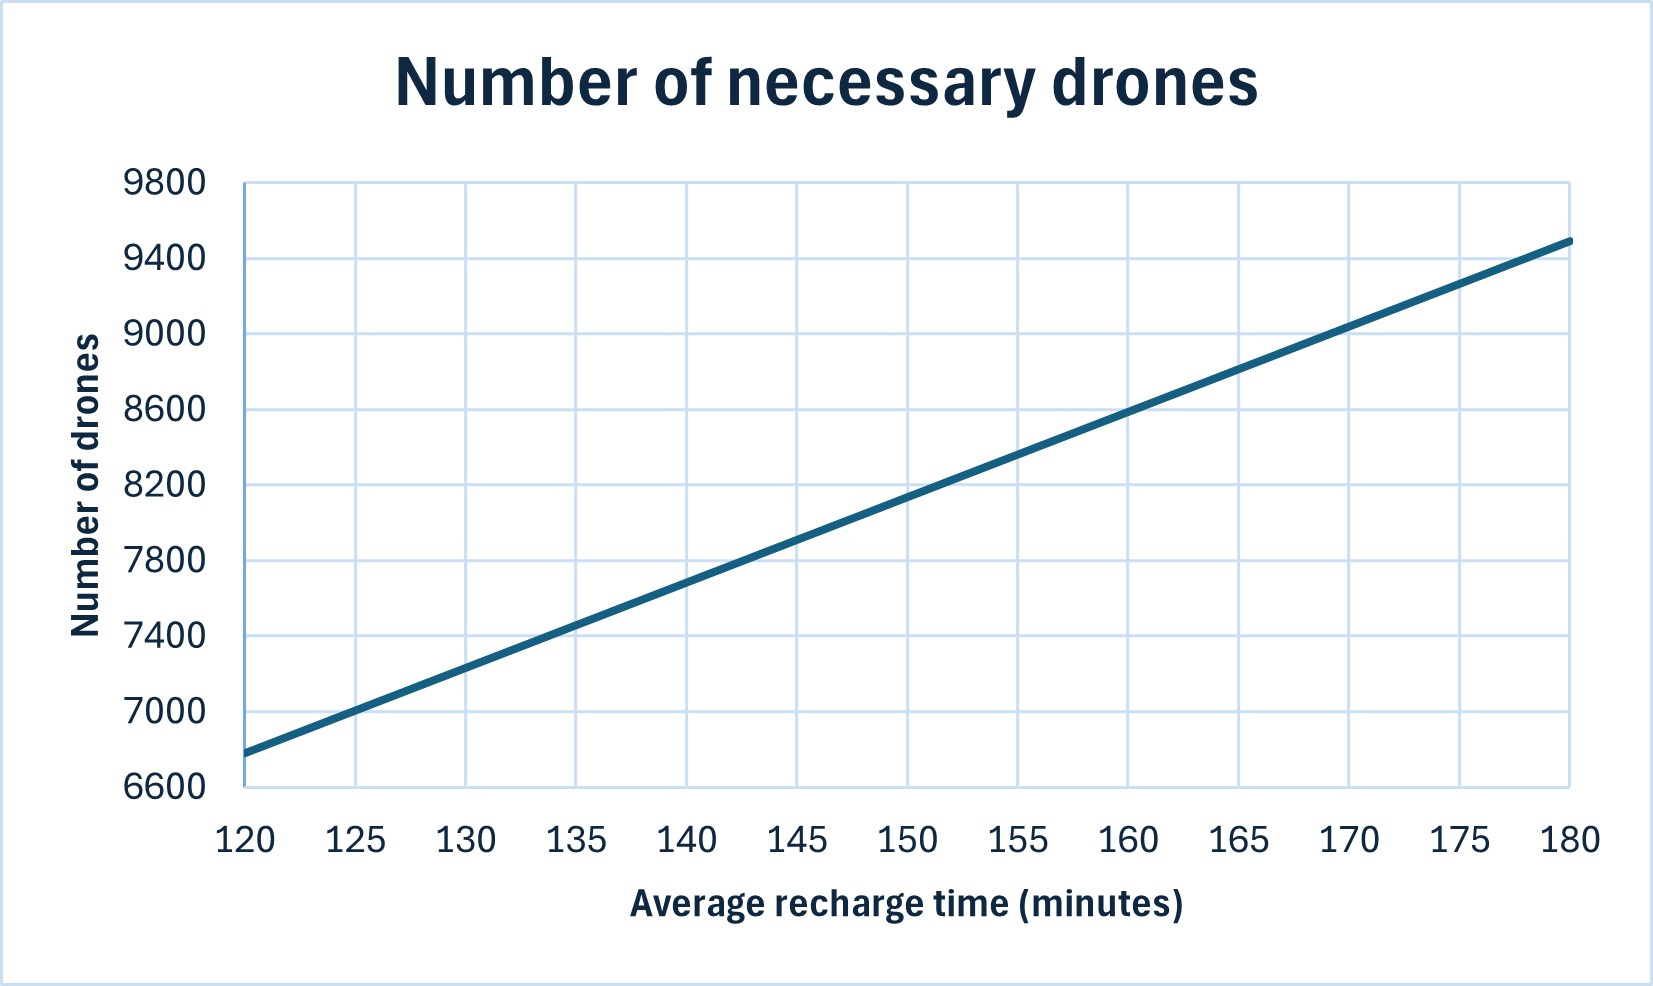
\includegraphics[width=0.9\textwidth]{nec_drones.png}
	\end{figure}
}
\newpage
\subsection{Conclusioni}
\raggedright\par{\large{
		L'implementazione del progetto \textbf{Sky Watch} ha permesso di raggiungere gli obiettivi preposti.\\}}
\vspace{10pt}
\raggedright\par{\large{
		I test effettuati hanno confermato che il sistema è in grado di raggiungere una copertura massimale dell'area e mantanerla per tutta la durata della sessione.\\
		I test dalle 12 alle 24 ore hanno inoltre anche dimostrato la tenuta del sistema nel lungo termine.\\
		Infine il calcolo a priori dei percorsi minimizza il numero di droni necessari senza compromettere la continuità operativa.}}
\vspace{10pt}
\raggedright\par{\large{I requisiti sia funzionali che non funzionali sono stati soddisfatti, evidenziando l'efficacia della strategia di implementazione adottata.\\
	}}
\end{document}



